\subsubsection*{Process}

The problem consists of two parts: implementing uniform sampling on
the unit disk and using these samples to implement a perspective
camera with depth of field.

\textbf{1) Uniform disk sampling: computing the PDF.}

Because we are working with a uniform distribution, the PDF should
be constant. Moreover, we know that it should integrate to 1 over
our domain.

Denoting the constant density by $c$, the integral over the unit disk
after conversion to polar coordinates is
\[
\int_0^1 \int_0^{2\pi}
p(r\cos\theta,r\sin\theta)\,r\,d\theta\,dr
= \pi c = 1.
\]

Therefore, the PDF is
\[
p(x,y) =
\begin{cases}
\frac{1}{\pi}, & x^2 + y^2 \leq 1,\\
0, & \text{otherwise}.
\end{cases}
\]

\textbf{2) Applying the multidimensional inversion method.}

In polar coordinates, the joint PDF is
$p_{r,\theta}(r,\theta)=r/\pi$.
The CDF, for $0\leq r_0\leq 1$ and $0\leq\theta_0\leq 2\pi$, is
\[
F(r_0,\theta_0)
= \int_0^{r_0} \int_0^{\theta_0}
\frac{r}{\pi}\,d\theta\,dr
= \frac{r_0^2\theta_0}{2\pi}.
\]

First, we compute the marginal CDF of $r$:
\[
F_r(r_0) = F(r_0,2\pi)
= \int_0^{r_0} \int_0^{2\pi}
\frac{r}{\pi}\,d\theta\,dr
= r_0^2.
\]

Applying the inverse CDF:
\[
r_i = F_r^{-1}(u) = \sqrt{u}.
\]

Next, we compute the conditional CDF of $\theta$ given $r_i$.
Since $p_r(r)=2r$, the conditional PDF for $r_i>0$ is
\[
p_{\theta|r}(\theta\mid r_i)
= \frac{p_{r,\theta}(r_i,\theta)}{p_r(r_i)}
= \frac{1}{2\pi}.
\]
Therefore,
\[
F_{\theta|r}(\theta\mid r_i)
= \int_0^\theta \frac{1}{2\pi}\,d\phi
= \frac{\theta}{2\pi}.
\]

Applying the inverse conditional CDF:
\[
\theta_i = F_{\theta|r}^{-1}(v\mid r_i) = 2\pi v.
\]
At $r_i=0$, the angle does not affect the resulting point.

Thus, for independent uniform samples $u,v\in[0,1]$, the resulting
transformation to Cartesian coordinates is
\[
\boxed{
(x_i,y_i)
= (r_i\cos\theta_i,\,r_i\sin\theta_i)
= \left(\sqrt{u}\cos(2\pi v),\,\sqrt{u}\sin(2\pi v)\right).
}
\]

The implementation directly follows this transformation. The PDF
function returns $1/\pi$ inside the unit disk and zero outside.

\lstinputlisting[
    language=C++,
    firstline=33,
    lastline=39,
    firstnumber=33
]{../../assignments/util/warp.cpp}

\begin{figure}[htbp]
    \centering
    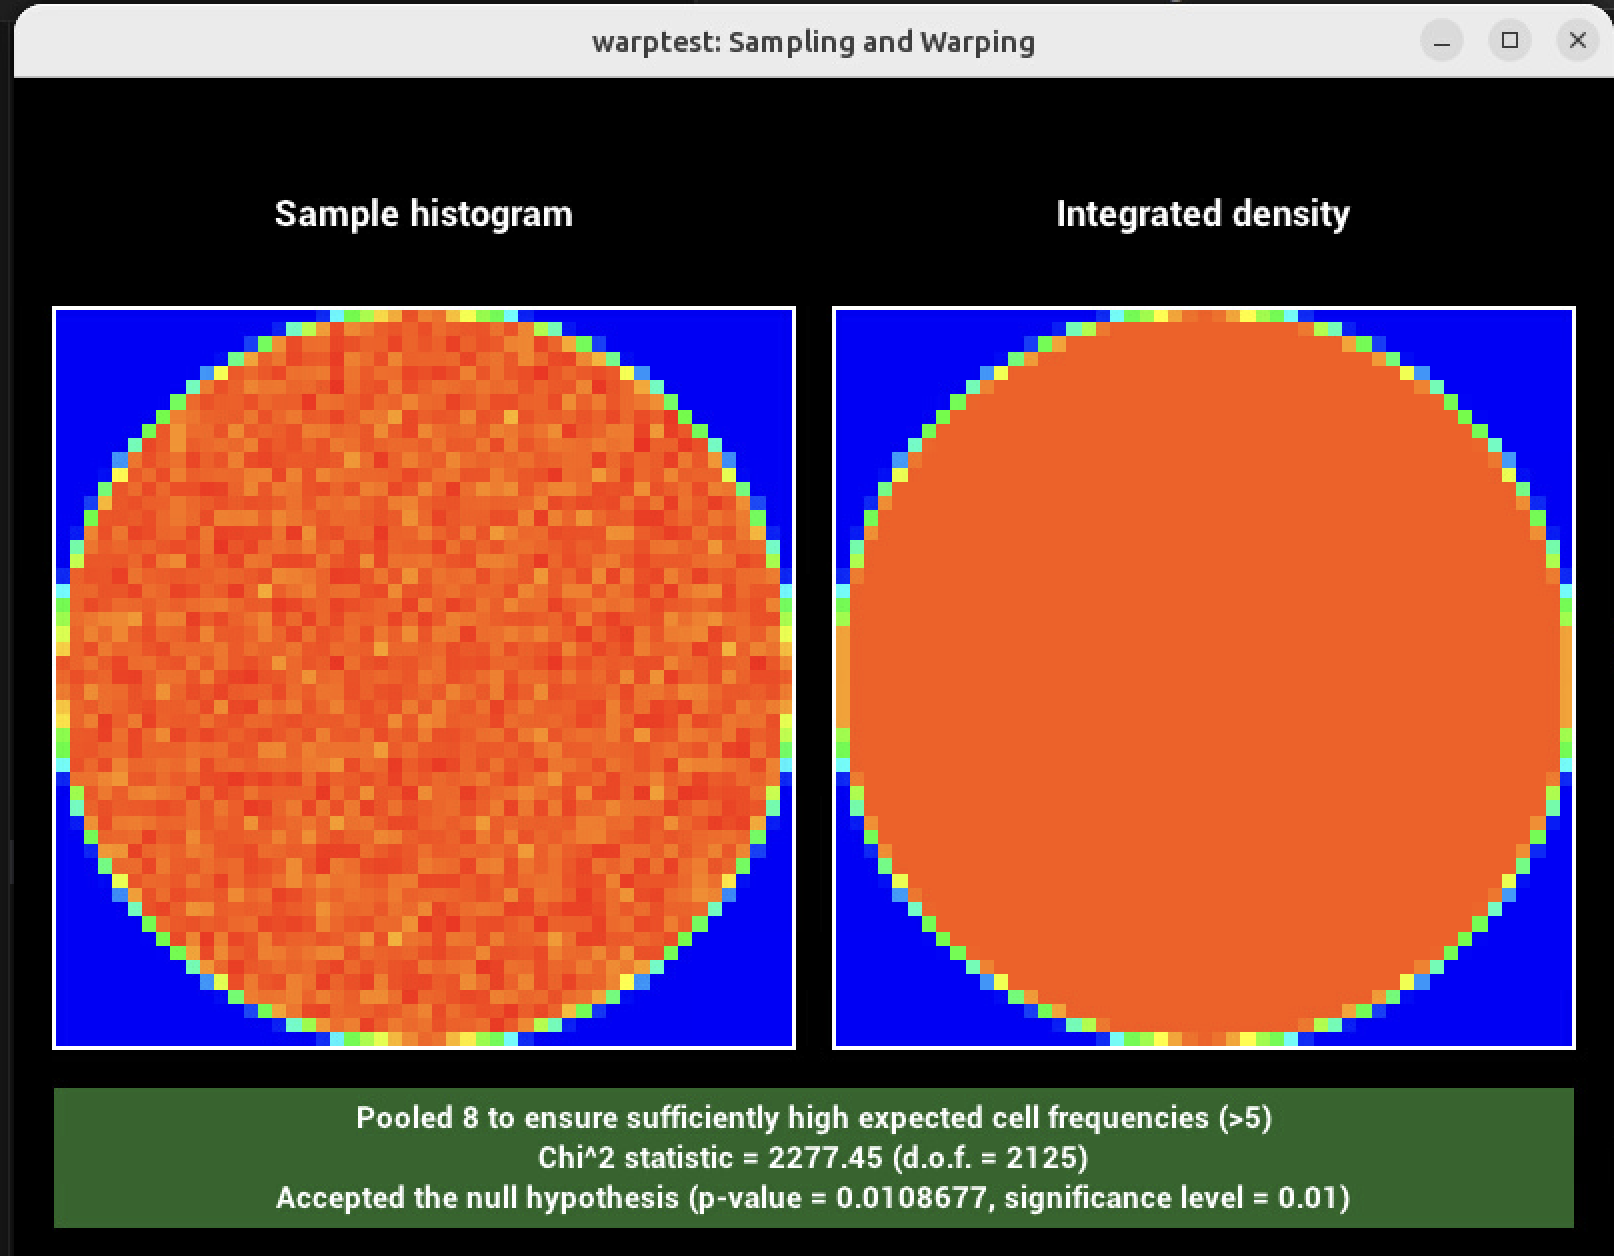
\includegraphics[width=0.8\textwidth]{pictures/circle_warp_test.png}
    \caption{Uniform disk sampling evaluated in the warptest application.}
\end{figure}

\textbf{3) Implementing the depth-of-field camera.}

We extend the perspective camera by adding a circular aperture and
a focus distance. For each image sample, we first find where the
original pinhole ray intersects the focus plane. We then sample
a point on the aperture using our uniform disk sampling function
and use it as the new ray origin. The ray is directed toward the
previously computed focus point.

Rays for the same image sample therefore meet at the same point
on the focus plane, keeping objects there sharp while blurring
objects in front of or behind it. Finally, we transform the ray
to world space and update its clipping interval.

\lstinputlisting[
    language=C++,
    firstline=211,
    lastline=242,
    firstnumber=211
]{../../assignments/camera/perspective.cpp}


\begin{figure}[htbp]
    \centering
    \begin{minipage}{0.32\textwidth}
        \centering
        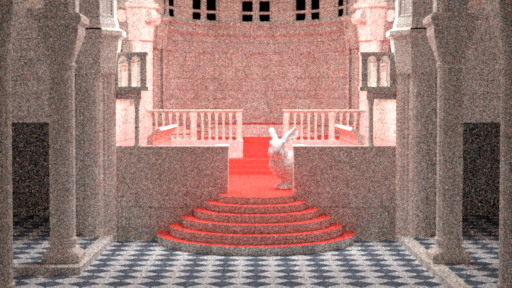
\includegraphics[width=\linewidth]{pictures/sibenik-path.png}
        \par\small Pinhole camera
    \end{minipage}
    \hfill
    \begin{minipage}{0.32\textwidth}
        \centering
        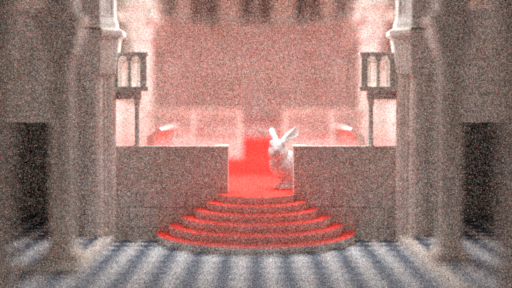
\includegraphics[width=\linewidth]{pictures/sibenik-path-dof.png}
        \par\small Depth-of-field camera
    \end{minipage}
    \hfill
    \begin{minipage}{0.32\textwidth}
        \centering
        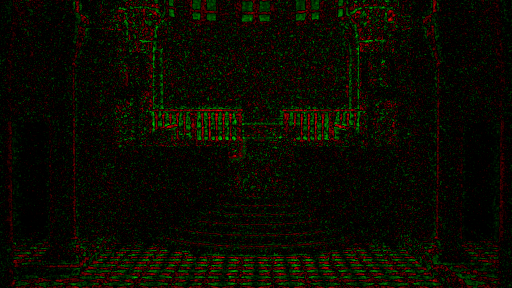
\includegraphics[width=\linewidth]{pictures/sibenik-path-comp.png}
        \par\small Comparison
    \end{minipage}
    \caption{Sibenik renders showing the depth-of-field effect.}
\end{figure}